\documentclass{article}
\usepackage{tikz}
\usetikzlibrary{shapes,matrix,positioning,arrows.meta,shapes.geometric}
\begin{document}
\begin{figure}
  \centering
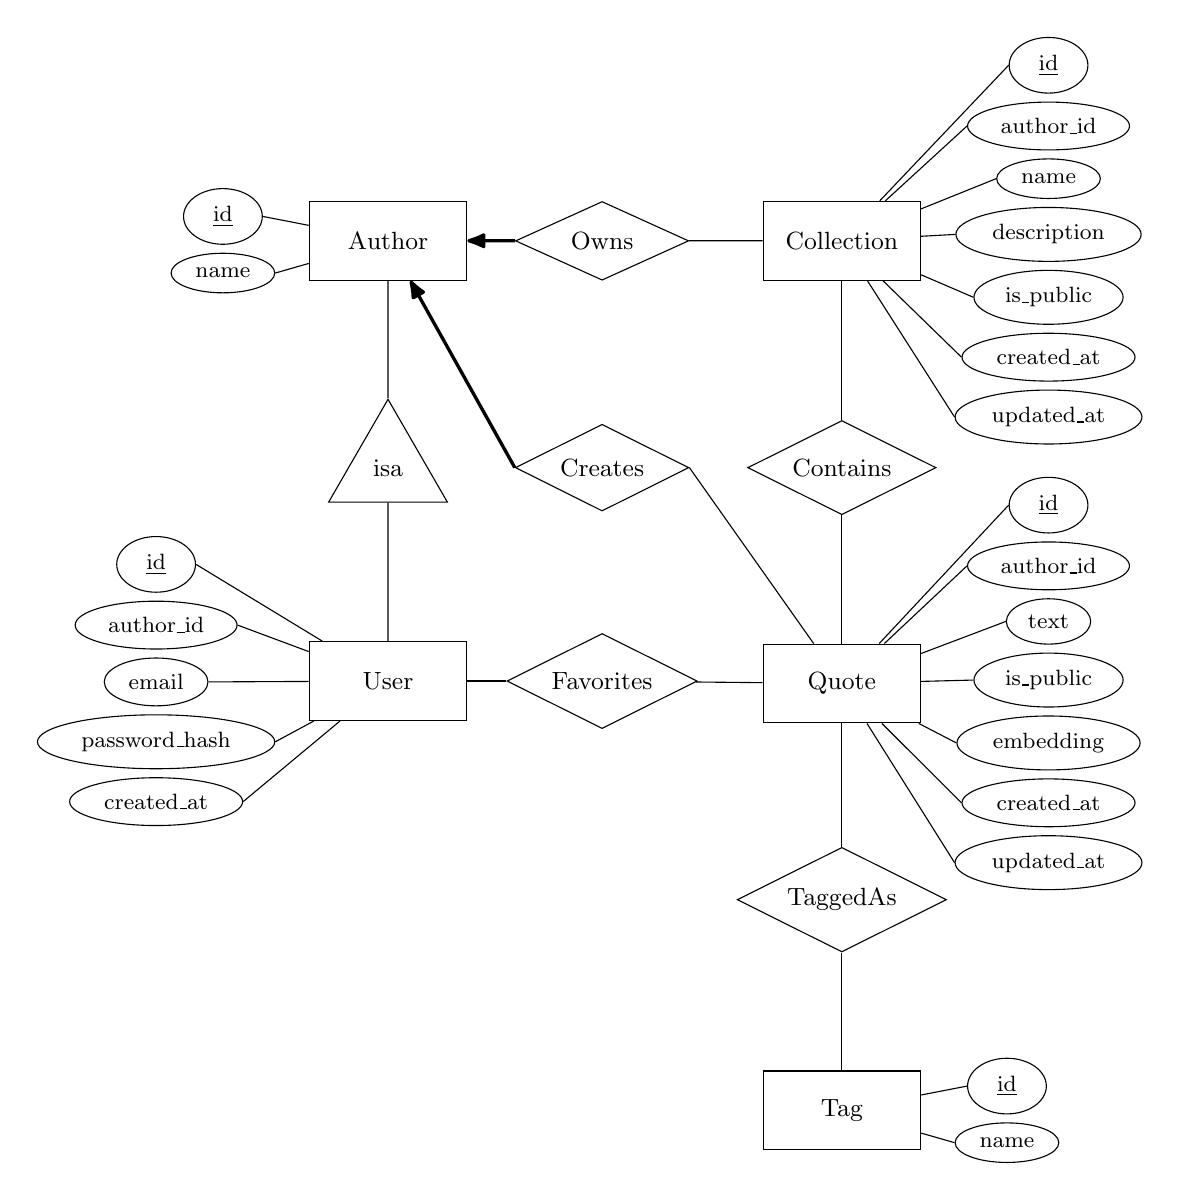
\begin{tikzpicture}
  % Settings
  \tikzset{
    attr/.style={draw, shape=ellipse, minimum width=1cm, minimum height=.5cm, align=center, font=\footnotesize},
    ent/.style={draw, shape=rectangle, minimum width=2cm, minimum height=1cm, align=center, font=\small},
    weak/.style={double,double distance=2pt},
    isa/.style={draw, regular polygon, regular polygon sides=3, minimum width=1cm, minimum height=1cm, align=center, font=\small},
    rel/.style={draw, shape=diamond, aspect=2, minimum width=2.2cm, text centered, align=center, font=\small},
    entrelgrid/.style={matrix of nodes, row sep=1.5cm, column sep=.5cm, nodes={ent}},
    attrib/.style={matrix of nodes, row sep=.1cm, column sep=.5cm, nodes={attr}},
  }
  \matrix (m) [entrelgrid]{
    \node[name=author] {Author};&\node[rel,name=owns] {Owns};           & \node[name=collection] {Collection};\\
    \node[isa,name=isa] {isa};  &\node[rel,name=creates]{Creates};      & \node[rel,name=contains] {Contains};\\
    \node[name=user] {User};    &\node[rel,name=favorites] {Favorites}; & \node[name=quote] {Quote};          \\
                                &                                       & \node[rel,name=taggedas] {TaggedAs};\\
                                &                                       & \node[name=tag] {Tag};              \\
  };
  % Arrows
  \draw[very thick, -{Latex[round]}] (owns) -- (author);
  \draw[very thick, -{Latex[round]}] (creates.west) -- (author);
  \draw (isa) -- (author);
  \draw (isa) -- (user);
  \draw (owns) -- (collection);
  \draw (contains) -- (collection);
  \draw (contains) -- (quote);
  \draw (creates.east) -- (quote);
  \draw (taggedas) -- (quote);
  \draw (favorites) -- (quote);
  \draw (favorites) -- (user);
  \draw (taggedas) -- (tag);
  % Author attributes
  \matrix (m1) [attrib,left=.3cm of author]{\underline{id}\\name\\};
  \foreach \i in {1,2} {\draw (m1-\i-1.east) -- (author);}
  % User attributes
  \matrix (m2) [attrib,left=.3cm of user]{\underline{id}\\author\_id\\email\\password\_hash\\created\_at\\};
  \foreach \i in {1,2,3,4,5} {\draw (m2-\i-1.east) -- (user);}
  % Collection attributes
  \matrix (m3) [attrib,right=.3cm of collection]{\underline{id}\\author\_id\\name\\description\\is\_public\\created\_at\\updated\_at\\};
  \foreach \i in {1,2,3,4,5,6,7} {\draw (m3-\i-1.west) -- (collection);}
  % Quote attributes
  \matrix (m4) [attrib,right=.3cm of quote]{\underline{id}\\author\_id\\text\\is\_public\\embedding\\created\_at\\updated\_at\\};
  \foreach \i in {1,2,3,4,5,6,7} {\draw (m4-\i-1.west) -- (quote);}
  % Tag attributes
  \matrix (m5) [attrib,right=.3cm of tag]{\underline{id}\\name\\};
  \foreach \i in {1,2} {\draw (m5-\i-1.west) -- (tag);}
\end{tikzpicture}
  \caption{The entity/relationship diagram for QuoteWeave.\label{fig:er}}
\end{figure}
The relations are shown below.
\texttt{Author(id:integer, name:text)}
\texttt{User(id:integer, author\_id:integer, email:text, password\_hash:text, created\_at:timestamptz)}
\texttt{Collection(id:integer, author\_id:integer, name:text, description:text, is\_public:boolean, created\_at:timestamptz, updated\_at:timestamptz)}
\texttt{Quote(id:integer, author\_id:integer, text:text, is\_public:boolean, embedding:vector, created\_at:timestamptz, updated\_at:timestamptz)}
\texttt{TaggedAs(quote\_id:integer, tag\_id:integer)}
\texttt{Tag(id:integer, name:text)}
\texttt{UserQuoteFavorite(user\_id:integer, quote\_id:integer, created\_at:timestamptz)}
\texttt{CollectionContains(collection\_id:integer, quote\_id:integer, added\_at:timestamptz)}
\end{document}